\documentclass[parskip=full]{scrartcl}
\usepackage[utf8]{inputenc} % use utf8 file encoding for TeX sources
\usepackage[T1]{fontenc}    % avoid garbled Unicode text in pdf
\usepackage[german]{babel}  % german hyphenation, quotes, etc
\usepackage{hyperref}       % detailed hyperlink/pdf configuration
\hypersetup{                % ‘texdoc hyperref‘ for options
pdftitle={SWT1: Lastenheftvorlage},%
}
\usepackage{graphicx}       % provides commands for including figures
\usepackage{csquotes}       % provides \enquote{} macro for "quotes"
\usepackage[nonumberlist]{glossaries}     % provides glossary commands
\usepackage{enumitem}

\makenoidxglossaries
%
% % Glossareinträge
%

\title{SWT1: Lastenheft}
\author{Oswald Zink, 2053536}

\begin{document}

\maketitle
\section{Zielbestimmung}
Die Firma Pear Corp. soll durch das Produkt iMage in der Lage sein Archivbilder zu speichern und zum Verkaufen anbieten zu k\"onnen. Die Bilder sollen dabei verschieden ausgegeben werden k\"onnen(e.g. Dateiformat, Gr\"osse)

\section{Produkteinsatz}
Das Produkt dient der Firma Pear Corp. zur Verwaltung, \"Anderung und Verkauf von Archivbildern.

Zielgruppe: Mitarbeiter der Firma Pear Corp. und Kunden.

Plattform: Betriebssystem mit Java Support.

\section{Funktionale Anforderungen}
\begin{itemize}[nosep]
\item[FA10] Speichern von Daten auf Firmen-internen Server.
\item[FA20] Hinzuf\"ugen und Entfernen von Bildern durch befugte Mitarbeiter.
\item[FA30] Hinzuf\"ugen und Entfernen von Schlagw\"ortern zu Bildern.
\item[FA40] Gew\"ahrleistet kleine Vorschaubilder f\"ur jedes Bild mit Wasserzeichen.
\item[FA50] Nutzer k\"onnen über eine Schlagwortsuche nach Bildern im Archiv suchen.
\item[FA60] Der Nutzer kann zwischen den Dateiformaten „JPG“, „PNG“ und „TIFF“ wählen.
\item[FA70] Der Nutzer kann den Kaufvorgang abbrechen.
\end{itemize}

\section{Produktdaten}
\begin{itemize}[nosep]
\item[PD10] Die Archivbilder sind zu speichern.
\item[PD20] Schlagw\"orter sind zu den Bildern zu speichern.
\item[PD30] Es sind relevante Daten \"uber die Kunden zu speichern.
\end{itemize}

\section{Nichtfunktionale Anforderungen}
\begin{itemize}[nosep]
\item[NF10] Die Schlagwortsuche dauert nicht l\"anger als 5 Sekunden.
\item[NF20] Die Schlagwortsuche liefert bis zu 10 nach Relevanz sortierte Bilder zur\"uck.
\item[NF30] Alle Bilder sind in den 3 Dateitypen: JPG, PNG und TIFF bereitgestellt.
\end{itemize}

\section{Systemmodelle}

\subsection{Szenarien}

\subsection{Anwendungsfälle}
\subsubsection{Seminarorganisation}
\begin{center}
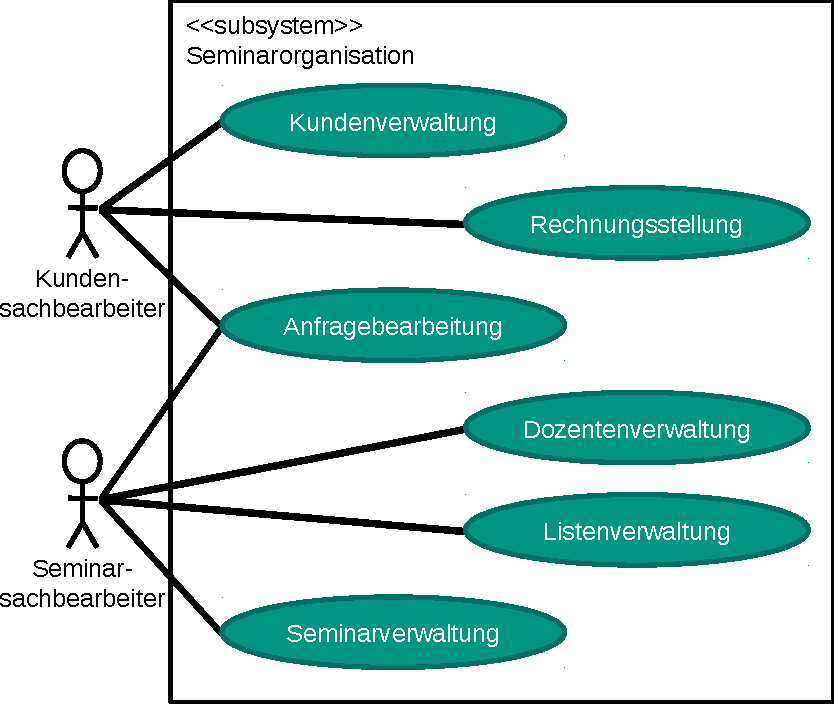
\includegraphics[width=0.8\textwidth]{szenario_seminarorganisation.pdf}
\end{center}

Akteure: Kundensachbearbeiter, Seminarsachbearbeiter.

Anwendungsfälle: Kundenverwaltung, Rechnungsstellung, Anfragebearbeitung, Dozentenverwaltung, Listenverwaltung, Seminarverwaltung.

Textuelle Beschreibung: (folgt)



%
% % Automatisch generiertes Glossar (Latex zwei mal ausführen um Glossar anzuzeigen)
%
%\glsaddall % das sorgt dafür, dass alles Glossareinträge gedruckt werden, nicht nur die verwendeten. Das sollte nicht nötig sein!
\printnoidxglossaries
Siehe \url{https://en.wikibooks.org/wiki/LaTeX/Glossary}.




\end{document}
